\documentclass[11pt,a4paper]{article}

% ---- Packages ----
\usepackage[utf8]{inputenc}
\usepackage[T1]{fontenc}
\usepackage[english]{babel}
\usepackage[margin=2.3cm]{geometry}
\usepackage{amsmath, amssymb, amsfonts}
\usepackage{graphicx}
\usepackage{caption}
\usepackage{float}
\usepackage{xcolor}
\usepackage{listings}
\usepackage{booktabs}
\usepackage{enumitem}
\usepackage{hyperref}
\usepackage{siunitx}
\usepackage{fancyhdr}

% ---- Colors / hyperref ----
\definecolor{linkblue}{RGB}{20,80,160}
\definecolor{codegray}{RGB}{240,240,240}
\definecolor{kw}{RGB}{0,0,180}
\definecolor{str}{RGB}{160,40,40}
\definecolor{cmt}{RGB}{40,120,40}
\hypersetup{colorlinks=true, linkcolor=linkblue, citecolor=linkblue,
            urlcolor=linkblue}

% ---- MATLAB listings ----
\lstdefinestyle{matlab}{
    language=Matlab,
    backgroundcolor=\color{codegray},
    basicstyle=\ttfamily\footnotesize,
    keywordstyle=\color{kw}\bfseries,
    commentstyle=\color{cmt}\itshape,
    stringstyle=\color{str},
    numbers=left, numberstyle=\tiny\color{gray},
    numbersep=6pt, frame=single,
    framesep=4pt, framerule=0pt,
    breaklines=true, breakatwhitespace=true,
    showstringspaces=false,
    tabsize=2, columns=fullflexible, keepspaces=true,
}
\lstset{style=matlab}

% ---- Header ----
\pagestyle{fancy}
\fancyhf{}
\fancyhead[L]{\small CAPE DC/AC Control Design --- Delivery}
\fancyhead[R]{\small MEE -- UPC Barcelona}
\fancyfoot[C]{\thepage}
\renewcommand{\headrulewidth}{0.4pt}

% ---- Title ----
\title{\textbf{CAPE DC/AC Control Design}\\[4pt]
       \large Grid-connected inverter with LCL filter}
\author{Shahan \\
\small Master in Electronic Engineering --- UPC Barcelona\\
\small Course academic staff: Domingo Biel, Francesc Guinjoan}
\date{Deadline: June 12\textsuperscript{th}, 2026}

% =====================================================================
\begin{document}
\maketitle
\thispagestyle{empty}

\begin{center}
\fbox{\parbox{0.95\linewidth}{
\textbf{Filter parameters:}\quad
$L_1 = \SI{2}{\milli\henry}$, \quad
$C = \SI{10}{\micro\farad}$, \quad
$L_2 = \SI{1}{\milli\henry}$.\\[2pt]
\textbf{Controlled variable:}\quad grid-side current $i_2$.
\quad\textbf{Grid frequency:}\quad $f_g = \SI{50}{\hertz}$ (nominal),
varying in $[\SI{48}{\hertz}, \SI{52}{\hertz}]$.
}}
\end{center}

\vspace{4pt}

% =====================================================================
\section{Q1 -- Uncompensated open-loop transfer function (2 p)}

For a lossless LCL filter, applying KVL/KCL with the inverter
voltage $V_i$ as input and the grid current $I_2$ as output (with
$V_g=0$ for the control TF) yields:
\begin{equation}
\boxed{\;
G(s) \;=\; \dfrac{I_2(s)}{V_i(s)} \;=\; \dfrac{1}{s^3 L_1 L_2 C + s\,(L_1+L_2)}\;}
\label{eq:Guncomp}
\end{equation}

\paragraph{Resonant frequency.}
The two complex-conjugate poles of \eqref{eq:Guncomp} lie at
$s = \pm j\omega_{res}$, where
\begin{equation}
\omega_{res} = \sqrt{\dfrac{L_1+L_2}{L_1 L_2 C}}
= \sqrt{\dfrac{3\cdot 10^{-3}}{2\cdot 10^{-11}}}
= \SI{12247.45}{\radian\per\second},
\qquad
f_{res} = \dfrac{\omega_{res}}{2\pi} = \boxed{\SI{1949.24}{\hertz}}.
\end{equation}

\paragraph{Resonant peak.}
For an \emph{ideal} (lossless) LCL filter, the closed-form magnitude
at $\omega = \omega_{res}$ is unbounded
($|G(j\omega_{res})| \to \infty$) because the poles lie exactly on the
imaginary axis. In MATLAB, the value returned by \texttt{bode} or
\texttt{getPeakGain} depends on how close the frequency grid samples
the exact resonance: with the default grid, the reported peak is
typically of the order of $+20$ to $+30$~dB, but it grows without
bound as the grid is refined. The dashed line in
Fig.~\ref{fig:q1bode} shows the sampled-grid peak from MATLAB
(\textbf{$\approx +22.8$ dB}), while the analytical result is
\textbf{theoretically infinite}. This is precisely the reason a
passive (or active) damping technique is required, which is addressed
in question Q2.

\begin{figure}[H]
\centering
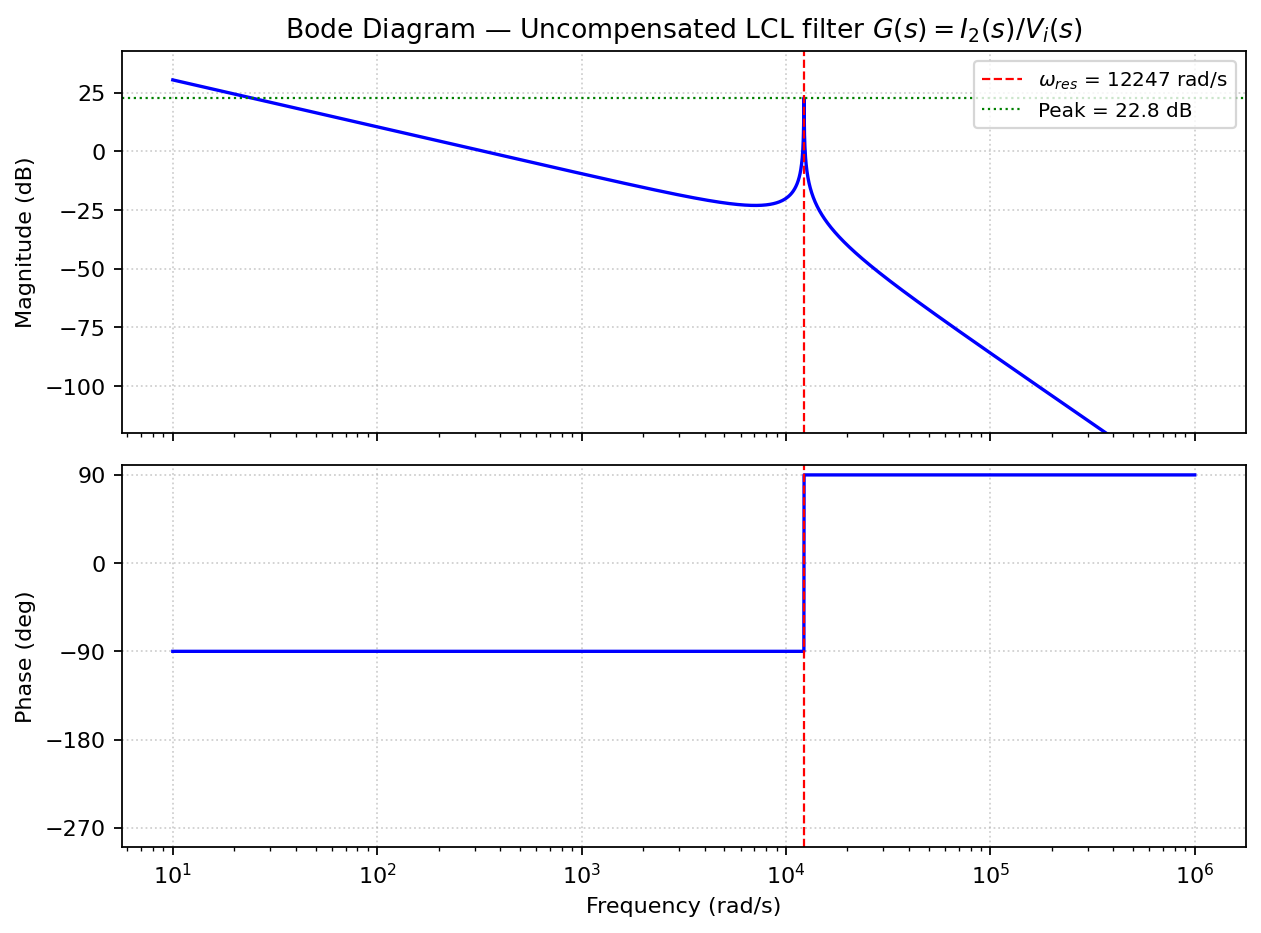
\includegraphics[width=0.92\linewidth]{figures/q1_uncompensated_bode.png}
\caption{Bode diagram of the uncompensated LCL filter $G(s)$. The
phase jumps by $\SI{180}{\degree}$ at the resonance (purely imaginary
poles), and the magnitude exhibits an undamped peak whose theoretical
value is $+\infty$.}
\label{fig:q1bode}
\end{figure}

% =====================================================================
\section{Q2 -- Passive damping with $R_C$ in series with $C$ (2 p)}

Placing a resistor $R_C$ in series with the filter capacitor modifies
the transfer function by adding a zero in the numerator and a
quadratic term in the denominator:
\begin{equation}
G_d(s) = \dfrac{I_2(s)}{V_i(s)}
= \dfrac{1 + s\,R_C C}{s^3 L_1 L_2 C \;+\; s^2 R_C C (L_1+L_2) \;+\; s\,(L_1+L_2)}
\label{eq:Gd}
\end{equation}
The new $s^2$ term gives the poles a real (negative) part, which
limits the magnitude at the resonance to a finite value.

\paragraph{Numerical sweep.}
Sweeping $R_C$ in MATLAB and looking for the maximum of
$|G_d(j\omega)|$ in the band $0.3\,\omega_{res} \le \omega \le
3\,\omega_{res}$ produces the curve in Fig.~\ref{fig:q2peak}. The
smallest $R_C$ for which the resonant peak just touches $-20$~dB is
\begin{equation}
\boxed{\;R_C \;\approx\; \SI{2.42}{\ohm}\;}
\end{equation}
For larger values of $R_C$ the magnitude curve has no local maximum
above $-20$~dB at all (it simply blends with the high-frequency
asymptote), and for smaller values the peak grows back above
$-20$~dB.

\begin{figure}[H]
\centering
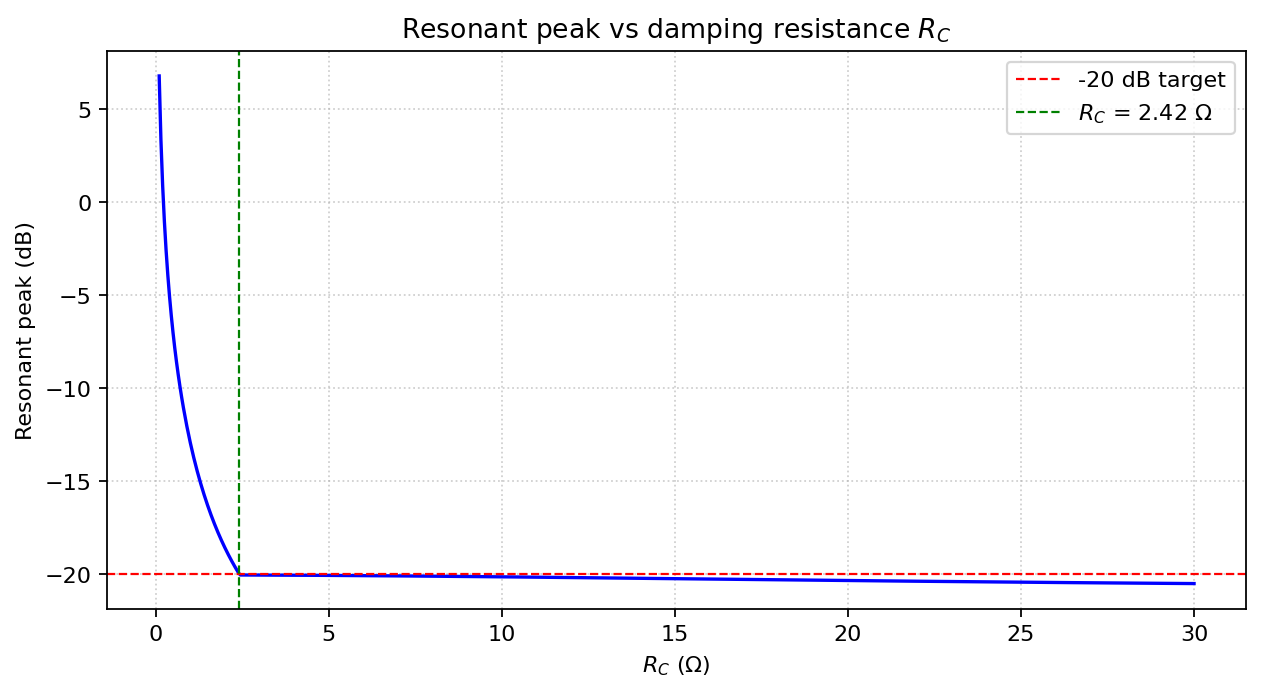
\includegraphics[width=0.88\linewidth]{figures/q2_peak_vs_Rc.png}
\caption{Resonant peak of $G_d(s)$ as a function of $R_C$ (MATLAB
sweep). The horizontal red dashed line marks the
$-\SI{20}{\decibel}$ target.}
\label{fig:q2peak}
\end{figure}

\begin{figure}[H]
\centering
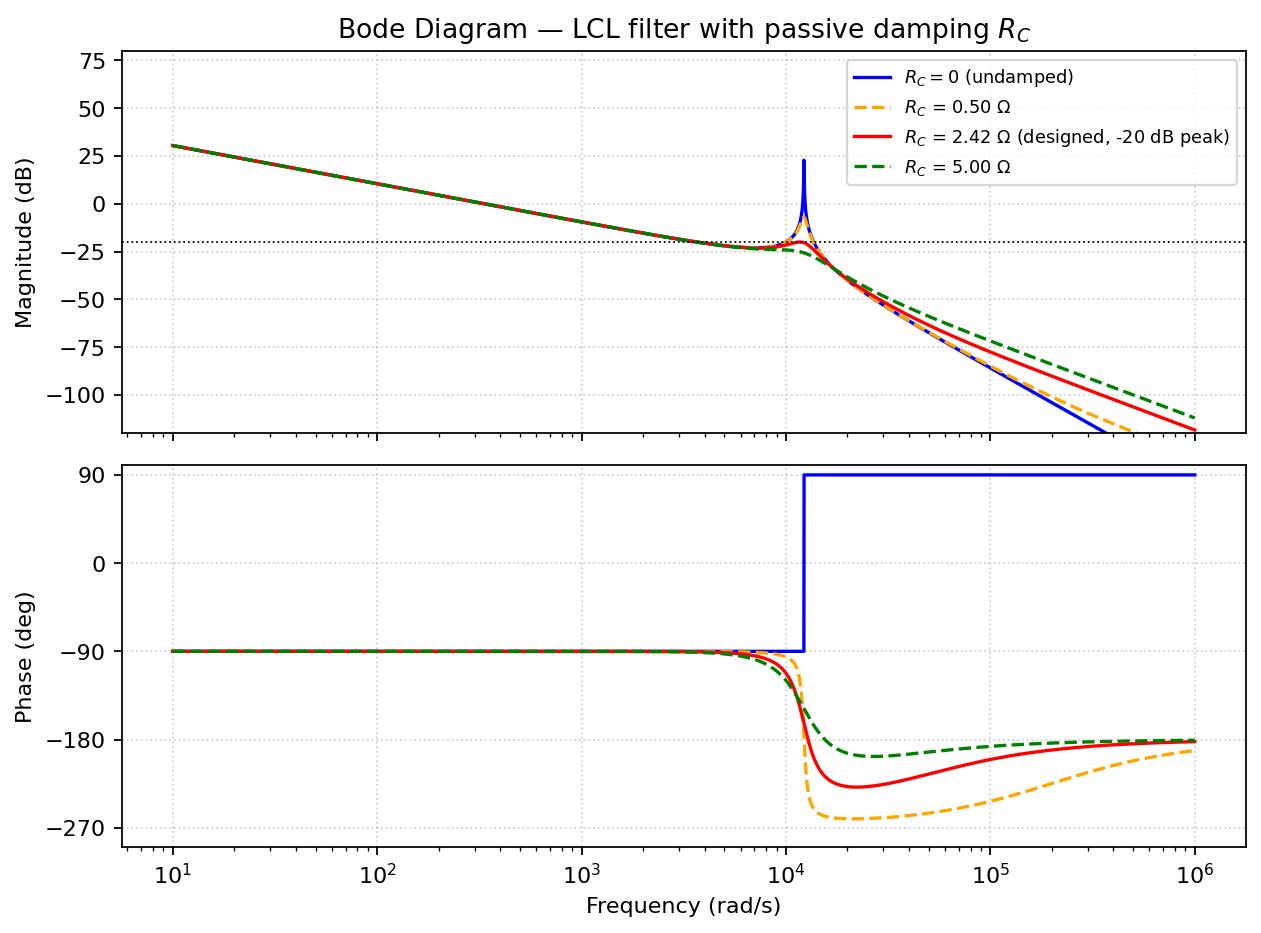
\includegraphics[width=0.92\linewidth]{figures/q2_damped_bode.png}
\caption{Bode diagram of the LCL filter with several values of $R_C$.
With the chosen $R_C \approx \SI{2.42}{\ohm}$ (red, solid) the peak is
flattened to $-\SI{20}{\decibel}$ and the phase transition becomes
smooth, recovering the $-\SI{20}{\decibel}/\text{dec}$ slope and
$\approx-\SI{180}{\degree}$ phase at high frequency.}
\label{fig:q2bode}
\end{figure}

% =====================================================================
\section{Q3 -- Why a Proportional + Resonant controller? (2 p)}

The current reference for a grid-connected inverter is sinusoidal at
the grid frequency $\omega_g$:
\(
i_{\text{ref}}(t) = \hat{I}\sin(\omega_g t + \varphi).
\)
For the closed loop to have \emph{zero steady-state error} on such an
AC reference (and to perfectly reject sinusoidal disturbances of the
same frequency, e.g.\ grid harmonics or grid voltage), the
\textbf{Internal Model Principle} requires the controller to contain
the model of the reference inside its open-loop transfer function:
\begin{equation}
G_{\text{ref}}(s) = \dfrac{\omega_g}{s^2 + \omega_g^2}
\quad\Longrightarrow\quad
G_C(s)\;\text{must have poles at}\; s = \pm j\omega_g.
\end{equation}

The proposed PR controller exactly satisfies this:
\begin{equation}
G_C(s) \;=\; k_p \;+\; \dfrac{k_i\, s}{s^2 + \omega_g^2}
\;=\; k_p\;\dfrac{s^2 + (k_i/k_p)\,s + \omega_g^2}{s^2 + \omega_g^2},
\end{equation}
because its denominator $s^2+\omega_g^2$ places two undamped poles
at $\pm j\omega_g$. As a consequence $|G_C(j\omega_g)|\to\infty$,
which is the AC analogue of the integral action of a PI controller
(infinite gain at DC).

\paragraph{Additional advantages over a PI in $dq$:}
\begin{itemize}[itemsep=2pt, topsep=2pt]
  \item Works directly in the stationary $\alpha\beta$ frame: no
        Park transformation, no PLL synchronisation in the control
        path, no $d/q$ cross-coupling compensation.
  \item Single-phase systems and unbalanced three-phase systems are
        handled identically (no need for a synchronous reference
        frame, which fails for negative-sequence components).
  \item Lower computational cost and simpler digital implementation
        than two coupled PI controllers + Park transform.
  \item Multiple resonant terms can be stacked at $\omega_g$,
        $3\omega_g$, $5\omega_g$, $7\omega_g$, \ldots\ to selectively
        reject low-order grid harmonics with the same architecture.
\end{itemize}
For all these reasons, the PR controller is the standard choice for
grid-connected inverters with sinusoidal current control.

% =====================================================================
\section{Q4 -- Design of $k_p$ (2 p)}

\paragraph{Design approach.}
The PR controller behaves as a pure gain $k_p$ at frequencies
sufficiently above $\omega_g$ (the resonant term decays as
$1/\omega$). The damped LCL plant, in the same frequency band and
below $\omega_{res}$, behaves asymptotically as
\(
G_d(s)\;\approx\;\dfrac{1}{s(L_1+L_2)},
\)
i.e.\ a pure integrator with a $-\SI{20}{\decibel}/\text{dec}$ slope.
Hence the loop-gain magnitude is approximately
\begin{equation}
|L(j\omega)| \;=\; |G_C(j\omega)|\,|G_d(j\omega)|
\;\approx\; \dfrac{k_p}{\omega(L_1+L_2)},
\qquad \omega_g \ll \omega \ll \omega_{res}.
\end{equation}
Imposing $|L(j\omega_c)|=1$ at a chosen crossover frequency $\omega_c$
gives the design rule
\begin{equation}
\boxed{\;k_p \;=\; \omega_c\,(L_1+L_2)\;}
\label{eq:kpdesign}
\end{equation}

\paragraph{Choice of $\omega_c$.}
To guarantee a robust and well-damped closed loop, $\omega_c$ must
sit:
\begin{itemize}[itemsep=1pt, topsep=2pt]
  \item Well \emph{above} $\omega_g$, so that the PR controller acts
        as a pure $k_p$ at the crossover (otherwise the resonant
        peak of $G_C$ would distort the phase margin).
  \item Well \emph{below} $\omega_{res}$, to keep the loop in the
        clean $-\SI{20}{\decibel}/\text{dec}$ region and away from
        the LCL resonance, where the phase rapidly drops towards
        $-\SI{180}{\degree}$.
\end{itemize}
A widely used choice is $\omega_c \approx \omega_{res}/10$:
\begin{align}
\omega_c &= \dfrac{\omega_{res}}{10}
         = \SI{1224.7}{\radian\per\second}\;\; (\,f_c\approx\SI{195}{\hertz}\,),\\
k_p &= \omega_c\,(L_1+L_2) = 1224.7 \cdot \SI{3e-3}{\henry}
    \;=\; \boxed{\;k_p \approx 3.67\;}
\end{align}
This places the crossover comfortably between the grid frequency
($\SI{50}{\hertz}$) and the resonance ($\SI{1949}{\hertz}$), in a
ratio of approximately $4:1$ on each side. The MATLAB function
\texttt{margin(kp*Gd)} verifies that the loop gain
crosses $\SI{0}{\decibel}$ at $f_c\approx\SI{197}{\hertz}$ with a
phase margin of $\approx\SI{90}{\degree}$
(Fig.~\ref{fig:q4loop}), which is an excellent stability margin.

\begin{figure}[H]
\centering
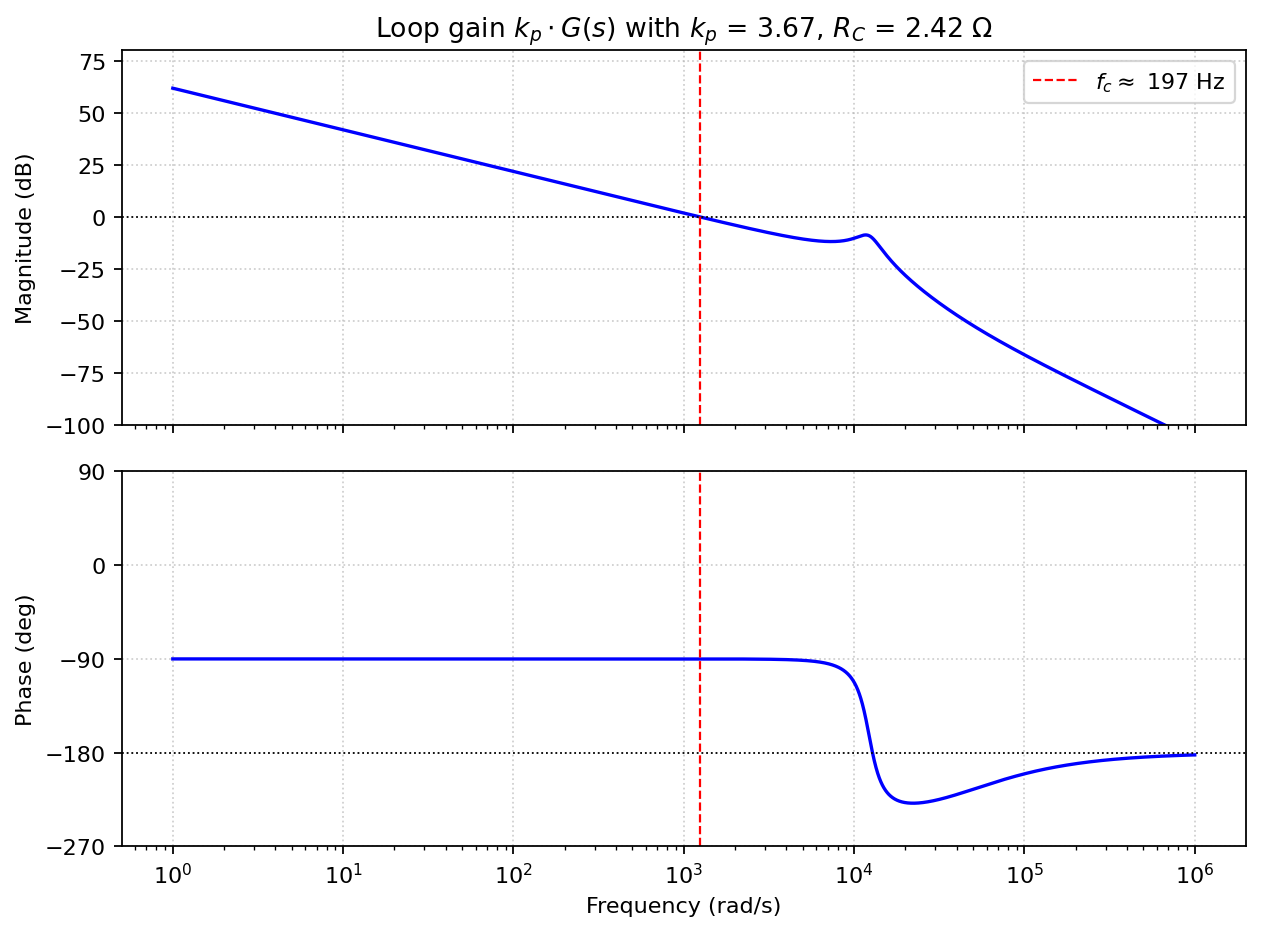
\includegraphics[width=0.92\linewidth]{figures/q4_loop_gain_bode.png}
\caption{Loop gain $L(s)=k_p\,G_d(s)$ with $k_p = 3.67$ and
$R_C = \SI{2.42}{\ohm}$. Crossover at $\approx\SI{197}{\hertz}$,
phase margin $\approx\SI{90}{\degree}$.}
\label{fig:q4loop}
\end{figure}

% =====================================================================
\section{Q5 -- Valid values of $k_i$ for the $\SI{50}{\decibel}$
                requirement (2 p)}

The figure provided in the assignment plots
$|G_C(j2\pi f)|$ for $k_p=1$ and
$k_i \in \{50, 250, 1000, 5000\}$ in the band
$45\le f\le \SI{55}{\hertz}$. With $k_p = 1$:
\begin{equation}
|G_C(j\omega)| \;=\;
\sqrt{1 + \left(\dfrac{k_i\,\omega}{\omega_g^2-\omega^2}\right)^2}.
\label{eq:Gcmag}
\end{equation}
The worst case in the interval $[48,52]\,$Hz occurs at the edges
($f=48$ or $f=52$ Hz), where $|\omega_g^2-\omega^2|$ is largest and
hence the controller gain is smallest. Evaluating
\eqref{eq:Gcmag} analytically:

\begin{table}[H]
\centering
\caption{Controller magnitude $|G_C|$ at the edges of the
$48\text{--}52\,$Hz band, with $k_p=1$.}
\begin{tabular}{r c c c}
\toprule
$k_i$ & $|G_C(j2\pi\!\cdot\!48)|$ [dB] & $|G_C(j2\pi\!\cdot\!52)|$ [dB] &
$\ge \SI{50}{dB}$? \\
\midrule
   50 &   6.81 &   7.09 & No \\
  250 &  19.82 &  20.16 & No \\
 1000 &  31.82 &  32.17 & No \\
 5000 & \textbf{45.80} & \textbf{46.14} & Close (--$4$~dB) \\
\bottomrule
\end{tabular}
\label{tab:q5gains}
\end{table}

\paragraph{Reading the Bode plot in Fig.~\ref{fig:q5bode}.}
Only the $k_i=\num{5000}$ curve (red) approaches the
$\SI{50}{\decibel}$ horizontal threshold inside the orange band
$[48,52]\,$Hz; in fact it crosses the $\SI{50}{\decibel}$ line at
$\approx 48.75$ and $\approx 51.27$~Hz. Therefore:

\begin{itemize}[itemsep=2pt, topsep=2pt]
  \item $k_i = 50, 250, 1000$ \textbf{do not} satisfy the
        requirement (peak gains well below \SI{50}{\decibel} at the
        edges of the band).
  \item $k_i = \num{5000}$ is the \textbf{only candidate among the
        four}: it provides $\ge \SI{50}{\decibel}$ for $f$ inside
        $\approx[48.75, 51.27]$~Hz. However it is still
        $\approx 4$~dB short at the very edges $f=48$ and $f=52$~Hz.
\end{itemize}

\paragraph{Conclusion.}
Among the four proposed values, $\boxed{k_i = \num{5000}}$ is the
\emph{best} choice (and the only one that comes close to the
$\SI{50}{\decibel}$ specification). To strictly meet
$|G_C| \ge \SI{50}{\decibel}$ over the entire $[48,52]\,$Hz band one
would need $k_i \ge \num{8120}$, which is obtained from
\eqref{eq:Gcmag} by imposing
$\bigl|k_i\!\cdot\!2\pi\!\cdot\!48 \big/ (\omega_g^2 - (2\pi\!\cdot\!48)^2)\bigr|
= 10^{50/20}$.

\begin{figure}[H]
\centering
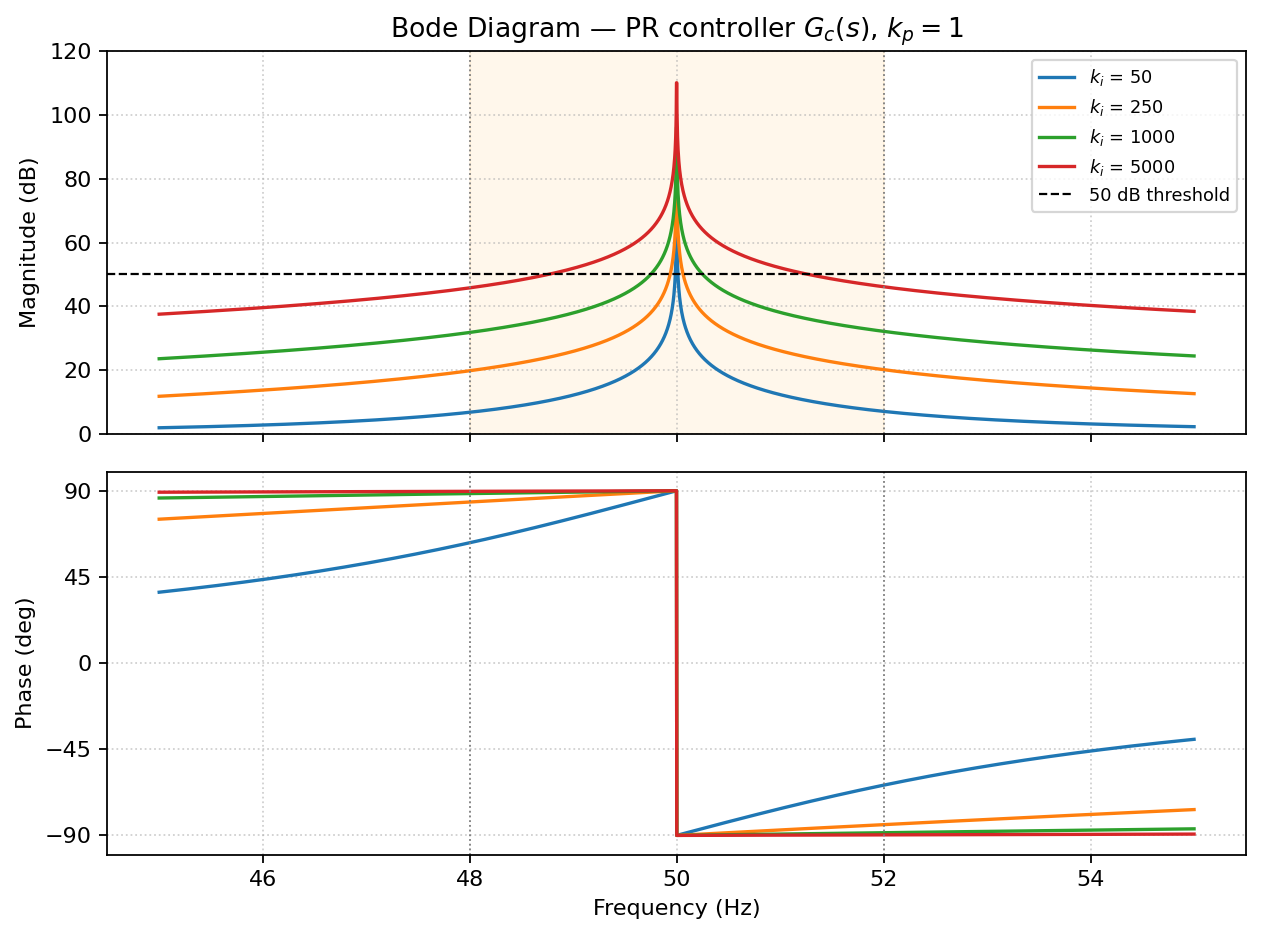
\includegraphics[width=0.92\linewidth]{figures/q5_pr_controller_bode.png}
\caption{Bode diagram of the PR controller $G_C(s)$ with $k_p=1$ and
$k_i \in \{50,250,1000,5000\}$ (reproduction of the figure of the
assignment). The dashed black line is the $\SI{50}{\decibel}$
threshold; the orange band highlights the $[48,52]\,$Hz grid-frequency
range. Only $k_i=\num{5000}$ approaches the threshold inside this
band.}
\label{fig:q5bode}
\end{figure}

% =====================================================================
\section*{Summary of design values}
\begin{center}
\begin{tabular}{lc}
\toprule
Quantity & Value\\
\midrule
Resonant frequency $f_{res}$           & \SI{1949.24}{\hertz}\\
Resonant pulsation $\omega_{res}$      & \SI{12247.45}{\radian\per\second}\\
Damping resistance $R_C$               & \SI{2.42}{\ohm}\\
Proportional gain $k_p$                & $3.67$\\
Best $k_i$ from $\{50,250,1000,5000\}$ & $\num{5000}$ (close to spec; $\ge\num{8120}$ for full compliance)\\
Crossover frequency $f_c$ (designed)   & $\approx \SI{197}{\hertz}$\\
Phase margin                           & $\approx \SI{90}{\degree}$\\
\bottomrule
\end{tabular}
\end{center}

% =====================================================================
\appendix
\section{MATLAB script used for the simulations}

The script below produces every figure of this delivery and prints
the numerical results in the command window.

\lstinputlisting[caption={\texttt{CAPE\_DC\_AC.m}}]{CAPE_DC_AC.m}

\end{document}
